\section{FCAL}
Most recent update: 2020-05-24 \\
Contact person: Wolfgang Lohmann (email: Wolfgang.Lohmann@desy.de)

\subsection{Introduction}
Two special electromagnetic calorimeters are foreseen in the very forward regions of a linear collider detector, denoted hereafter as
LumiCal and BeamCal. In front of BeamCal a layer of pixel detector, denoted as Pair Monitor, will support beam tuning.
\begin{figure}[hbp]
  \centering
   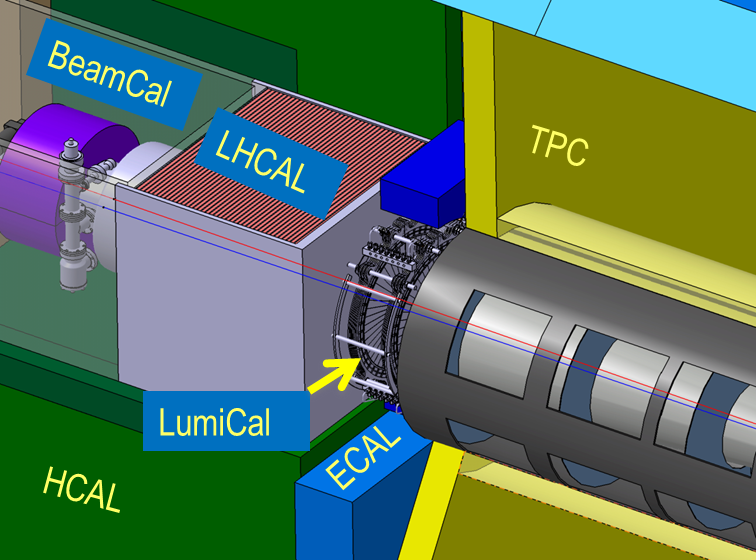
\includegraphics[width=0.45\columnwidth]{Calorimeter/FCAL/figs/forward_region_new} \hfill
   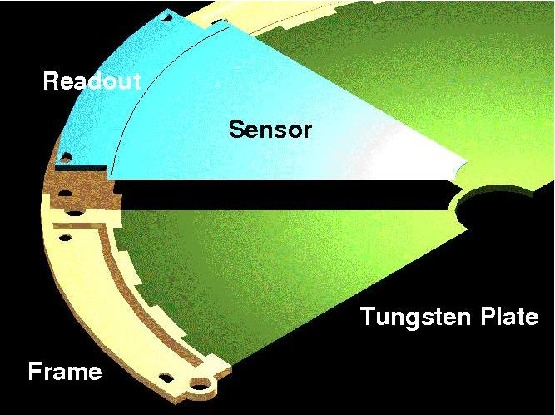
\includegraphics[width=0.45\columnwidth]{Calorimeter/FCAL/figs/BClayer}
  \caption{Left: The very forward region of the ILD detector.
  LumiCal, BeamCal and LHCAL are carried by
  the support tube for the final focusing quadrupole QD0 and the beam-pipe.
  TPC denotes the central track chamber, ECAL the electromagnetic and
  HCAL the hadron calorimeter.
  Right: A half layer of an absorber disk with a sensor sector and front-end electronics.}
  \label{fig:Forward_structure}
\end{figure}
These calorimeters will deliver both a fast and a precise measurement of the luminosity
and extend the detector coverage to low polar angles.
In addition, a LHCal extends the hadron calorimeter coverage to very small polar angles.
Detailed Monte Carlo studies have been performed to
optimize the design of the calorimeters, estimate the background from physics processes and understand the impact
of beam-beam interactions on the luminosity measurement~\cite{2010JInst...512002A}.
A sketch of the design is shown in Figure~\ref{fig:Forward_structure}~(left).

To ensure a high efficiency for single high energy electron detection on top of the large and widely spread
background from beamstrahlung, calorimeters with a small Moli\`{e}re radius are needed. Such compact calorimeters 
also ensure the necessary  precision in the angular reconstruction of Bhabha scattering events.

Due to the high occupancy originating from beamstrahlung and two-photon processes,
both calorimeters need a dedicated fast readout.
In addition, the lower polar angle range of BeamCal is exposed to a large flux
of low energy electrons, resulting in depositions up to one
MGy per year. Hence, radiation hard sensors are necessary.

Compact
cylindrical sandwich
calorimeters using tungsten absorber disks of one radiation length thickness, interspersed with
finely segmented silicon (LumiCal) or GaAs (BeamCal) sensor planes, as sketched in
Figure~\ref{fig:Forward_structure}~(right),
are found
to match the requirements from physics~\cite{2010JInst...512002A}.
LHCal will be designed with a small hadronic interaction length, to fit into the limited space available.

\subsection{Prototype Construction and Beam Tests}

\subsubsection{Currently used Sensors}

Large area GaAs sensors, as shown in Figure~\ref{fig:GaAs} (left), were developed
and produced in collaboration with partners in Russian industry. The Liquid Encapsulated
Czochralski technology is used. The sensors were
doped by a shallow donor (Sn or Te),
and then compensated  with Chromium.
\begin{figure}
\centering
    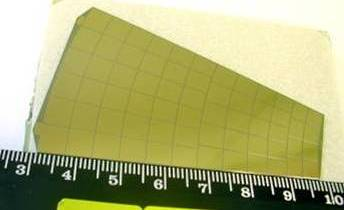
\includegraphics[width=0.4\columnwidth, height=4cm]{Calorimeter/FCAL/figs/GaAs_sensor_new.jpg}
    \hspace{1cm}
     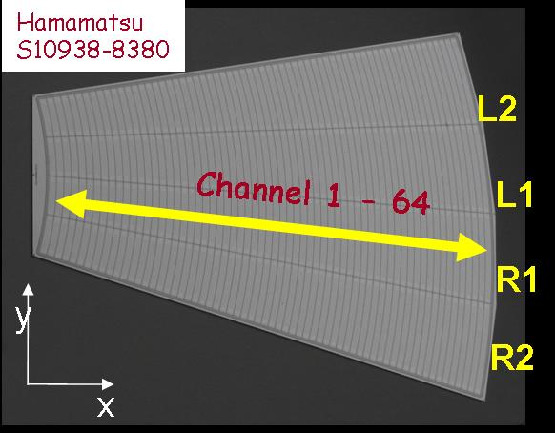
\includegraphics[width=0.4\columnwidth]{Calorimeter/FCAL/figs/si_proto.jpg}
          \caption{Left: A GaAs pad sensor developed for BeamCal, Right: A silicon pad sensor designed for LumiCal and manufactured by Hamamatsu Photonics.}
    \label{fig:GaAs}
\end{figure}
This results in a semi-insulating GaAs material with a resistivity of about \SI{e7}{\ohm \meter}.
The sensors are \SI{0.5}{mm} thick with pads of a few \si{\milli\meter\squared} area. The operation voltage is about \SI{100}{V} with
leakage current per pad less than \SI{500}{nA}.

Prototypes of LumiCal sensors have been designed
at the Institute of Nuclear Physics PAN
in Cracow~\cite{EUDETMEMO-2009-07} 
and manufactured by Hamamatsu
Photonics.
Their shape, as shown in Figure~\ref{fig:GaAs} (right), is a ring segment of 30\textdegree.
The thickness of the n-type silicon bulk is \SI{0.320}{mm}.
The pitch of the concentric p$^+$ pads is \SI{1.8}{mm} and
the gap between two pads is \SI{0.1}{mm}.
The bias voltage for full depletion ranges between 39 and \SI{45}{V},
and the leakage currents per pad are below \SI{5}{nA}.

\subsubsection{Development of Readout ASICs}

As a first step, dedicated ASICs were designed choosing
an
architecture~\cite{Boie1982365,Gatti:1986qq}
comprising a charge sensitive amplifier and a shaper.
ASICs, containing 8 front-end channels, were designed and fabricated in \SI{0.35}{\micro\meter} CMOS technology.
A variable gain in both the charge amplifier and
the shaper is implemented by a mode switch. The peaking time of the shaper output signal is \SI{60}{ns}.
More results of the measurements of the performance were published elsewhere~\cite{4600902}.
A dedicated low-power, small-area, multichannel ADC is designed and produced~\cite{6156491}.
It comprises eight 10-bit power and frequency (up to \SI{24}{MS/s}) scalable pipeline ADCs and the necessary
auxiliary components.
The readout system containing 32 channels (four pairs of 8-channel front-end and ADC ASICs) was developed and used
successfully in several test-beams, confirming that the chosen readout architecture fulfills the LumiCal requirements.
The main limitation of this ASICs was the number of channels, allowing to build only
small (32 readout channels)  prototype of detector modules. For this reason a new
development of LumiCal readout ASICs called FLAME (FcaL Asic for Multiplane rEadout)
was pursued. The block diagram of FLAME is shown in Figure~\ref{fig:FLAME}. 
\begin{figure}
\centering
    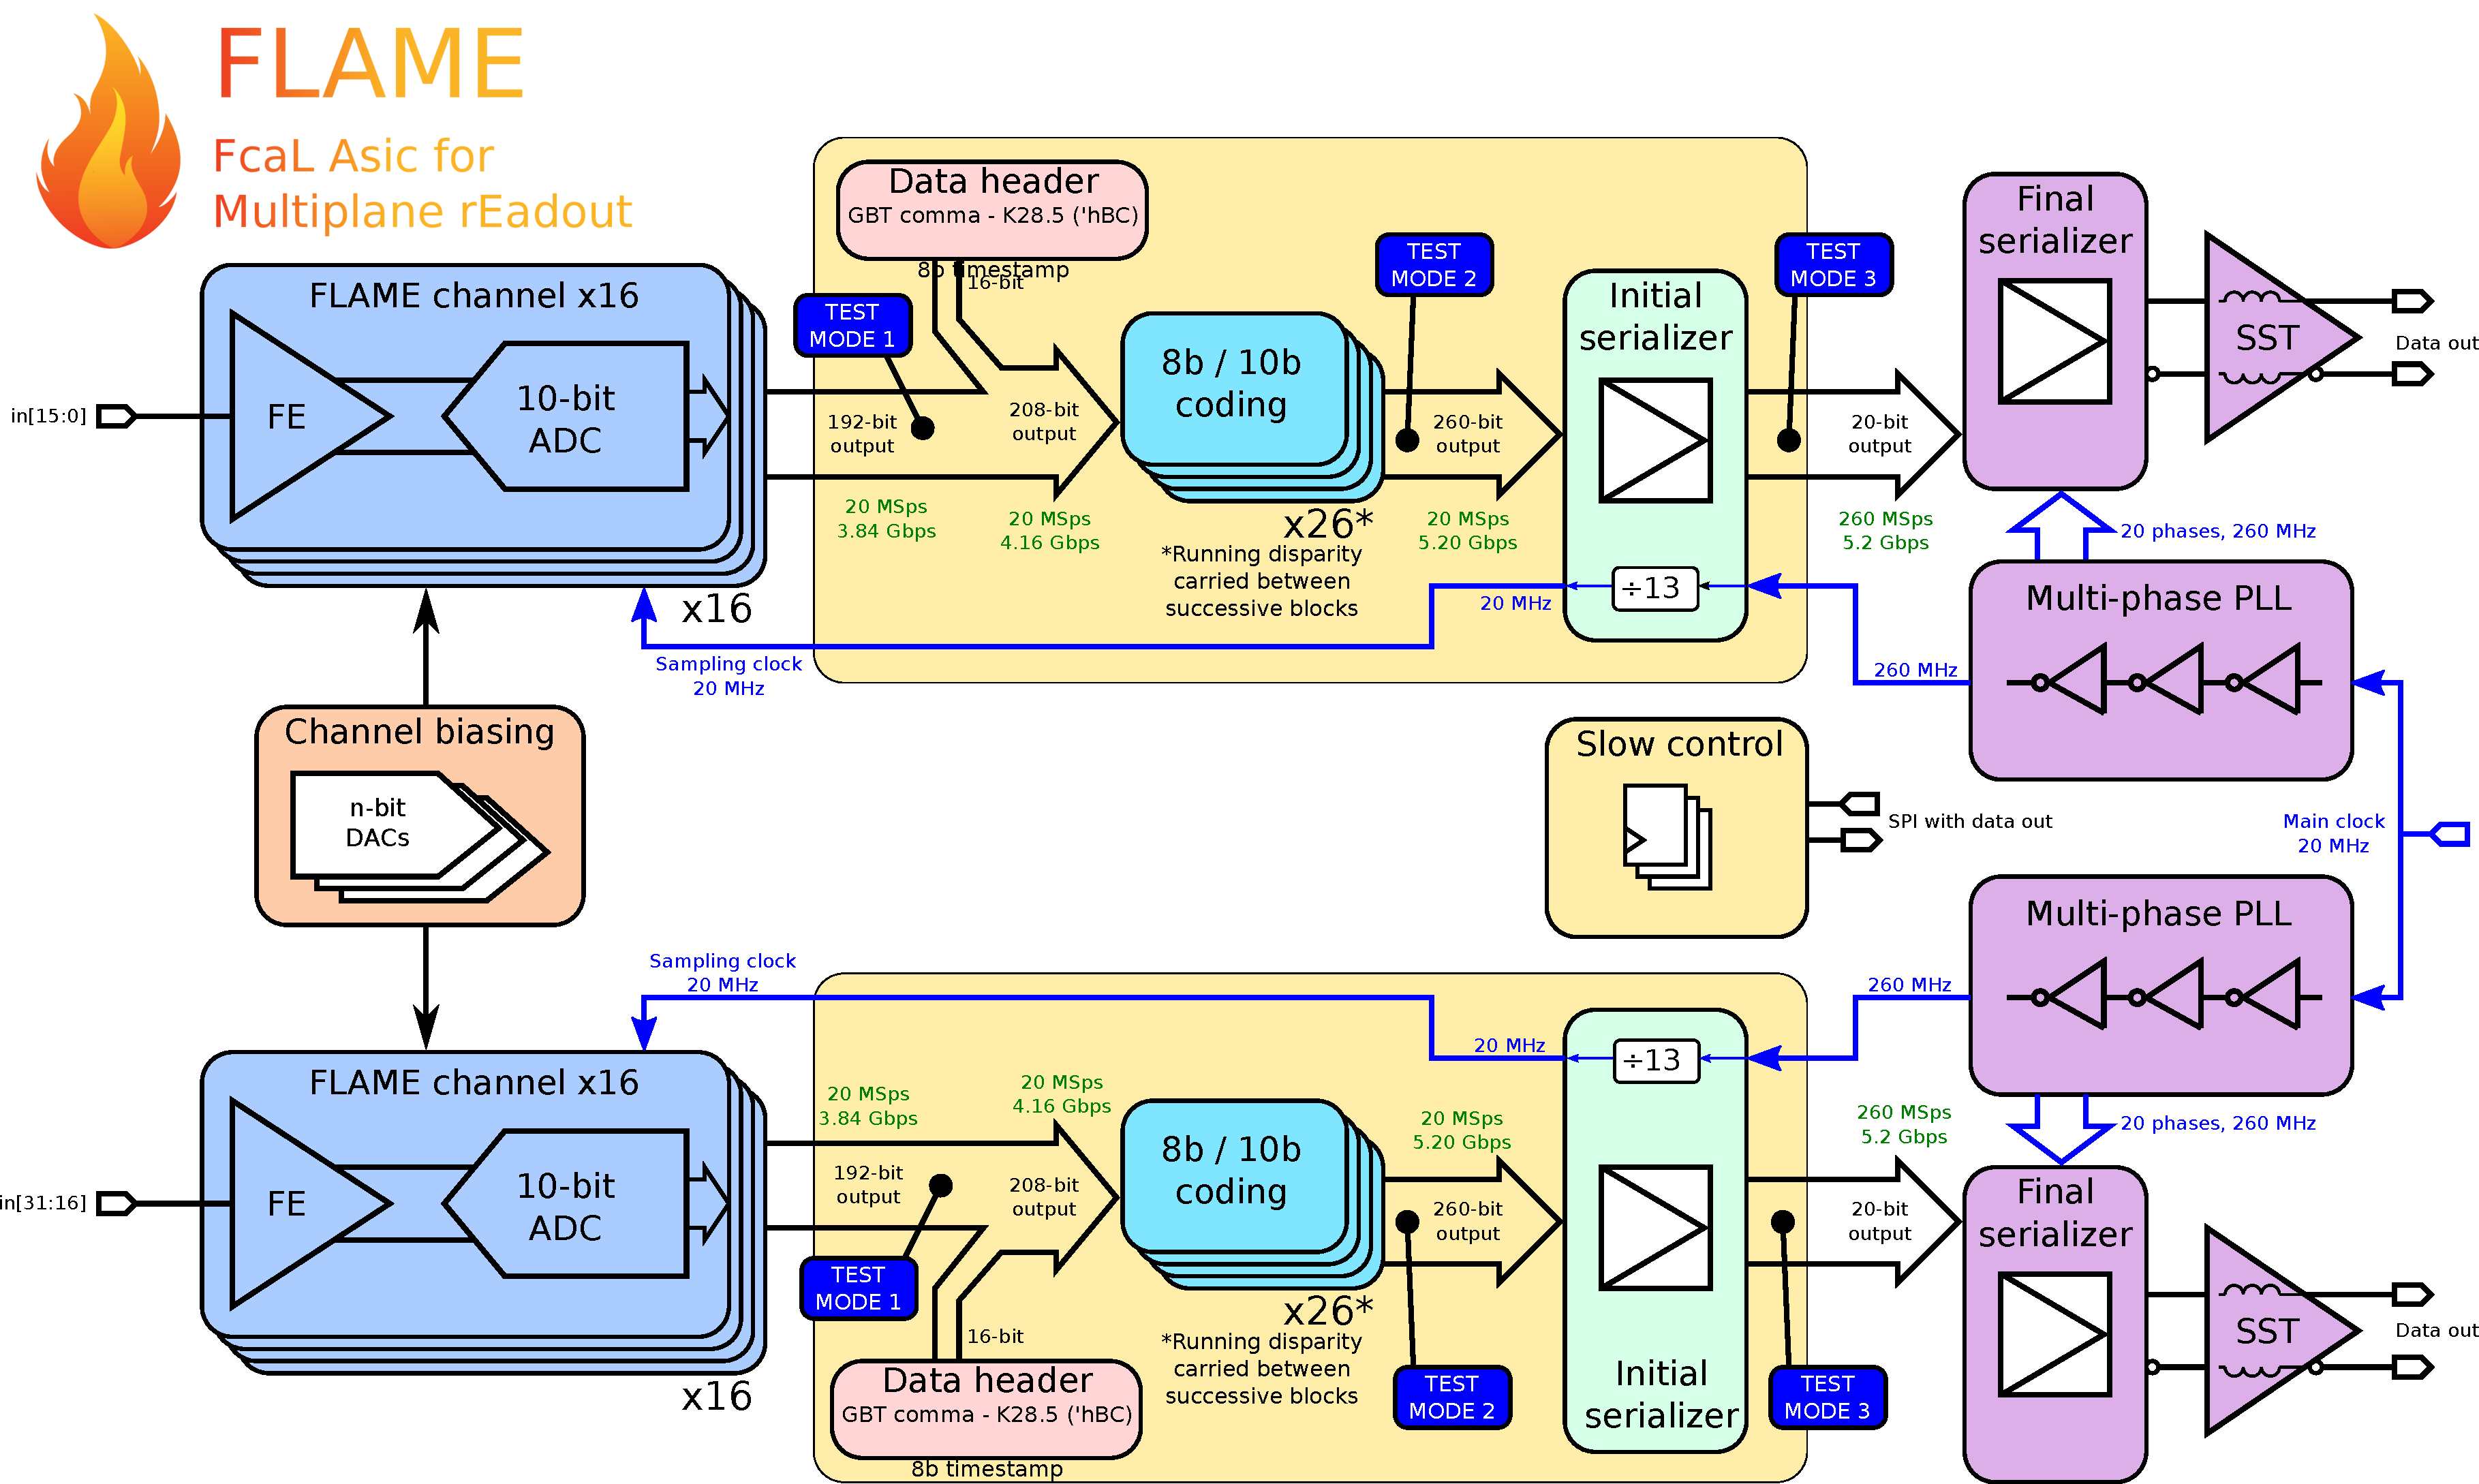
\includegraphics[width=0.9\columnwidth]{Calorimeter/FCAL/figs/FLAME}
    \caption{A block diagram of FLAME readout ASIC.}
    \label{fig:FLAME}
\end{figure}
The FLAME uses the same architecture as the previous readout, with analog front-end and 10-bit ADC in each channel.
The main differences and improvements are listed below. 
\begin{itemize}
\item{FLAME is developed in smaller size TSMC 130~nm CMOS technology.
 This choice allows to obtain large reduction of power consumption and much better radiation hardness}.
\item{FLAME is a System on Chip (SoC) solution comprising all functionality
  (analog front--end, ADC, data serialization and transmission) in one ASIC.
  It will simplify the architecture of the overall readout system and minimise the number of its components.}
\item{FLAME ASICs comprises 32-channels. Designing a readout board with 8 ASICs one can build a detector module
  reading the whole LumiCal sensor tile, containing 256 channels.}
\item{FLAME is built of two identical 16-channel blocks. The data from each block is sent out
  by a very fast (\SI{5.2}{Gbps}) serializer and serial data transmission block. The output data is coded and formatted so that it may be directly received by fast FPGA links.}
\end{itemize}
The development of FLAME has been recently completed. The laboratory tests confirmed that all performance parameters have been matched. Readout boards equipped with FLAME ASICs have been used recently in test-beam measurements of a LumiCal prototype.  

\subsubsection{Data Concentrator and DAQ}

In order to operate a large amount of sensor planes the readout has to be orchestrated.
For this purpose a FPGA based data concentrator is developed.
The prototype of a DAQ module uses a Zynq UltraScale+ FPGA on a Trenz TE0808m board.
The module reads data sent by FLAME, processes and sends them to an external data store using ethernet transmission. 
The current architecture with the generated blocks inside the FPGA is shown in Figure~\ref{fig:FPGA_scheme}. 

\begin{figure}
\centering
    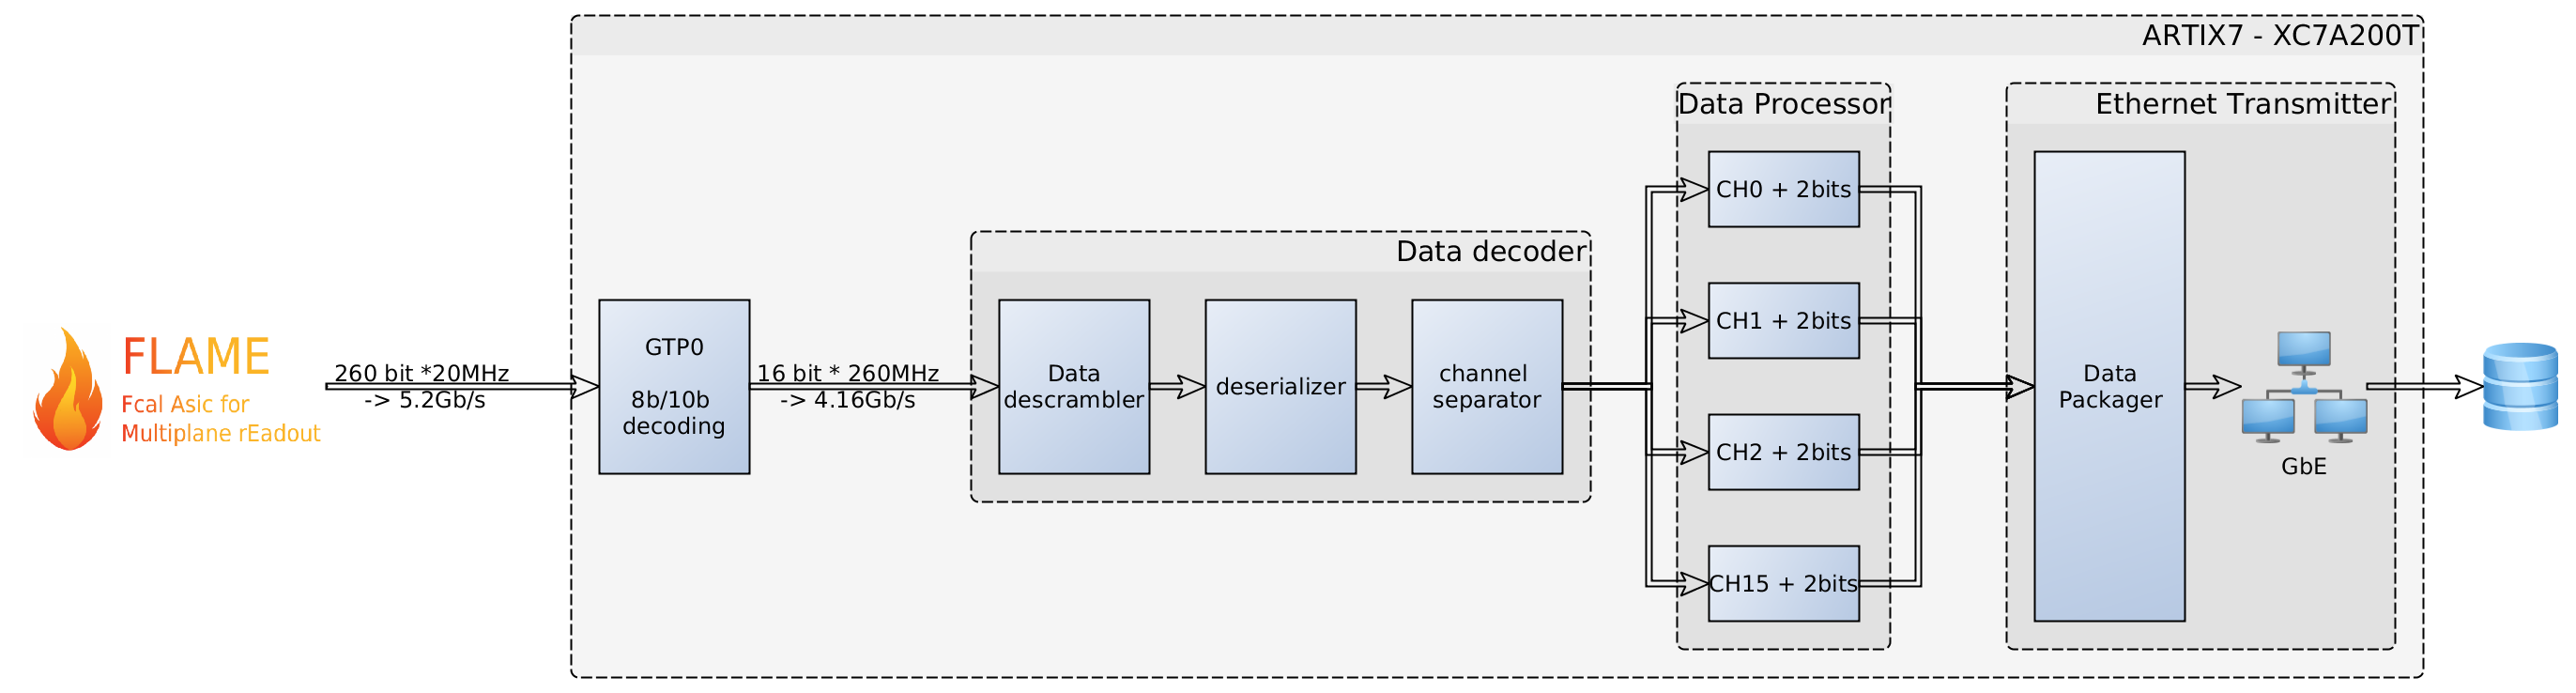
\includegraphics[width=\textwidth]{Calorimeter/FCAL/figs/FPGA_scheme} 
	\caption{Block diagram of the FPGA module used in test-beam measurements.}
    \label{fig:FPGA_scheme}
\end{figure}

\subsubsection{High Quality Tungsten Absorber Plates}

A batch of 25 absorber plates has been fabricated for JINR Dubna by partners in the Russian industry. 
The absorber composition is W 92.5\%, Ni 5.25\%, and Cu 2.25\%.
The material density is \SI{18.0}{\gram\per\centi\meter\cubed}. The thickness of the plates has been assessed using a Zeiss 3D coordinate
measurement system with a precision \SI{2.5}{\micro\meter}. Front and back side measurements were done. The deviation
from planarity is for most of the plates within \SI{50}{\micro\meter} as shown in Figure~\ref{fig:tungsten}.
\begin{figure}
  \centering
   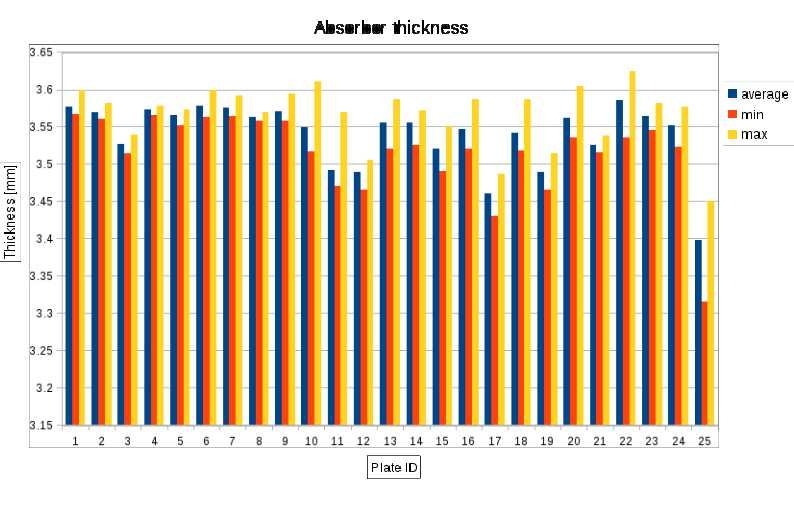
\includegraphics[width=0.9\columnwidth]{Calorimeter/FCAL/figs/tungsten_disk_thickness.jpeg} 
   \caption{Thickness of the tungsten absorber plates. Average thickness and minimum and maximum deviation from planarity is shown.}
  \label{fig:tungsten}
\end{figure}

\subsubsection{Mechanical Stack}

A flexible mechanical structure, as shown in Figure~\ref{fig:mechanical_structure}, has been 
built by CERN as part of the AIDA project,
to compose a technological 
calorimeter prototype instrumented both with LumiCal and BeamCal sensors. 
Tungsten absorber plates, glued on a permaglass
frame, are precisely
positioned on a rod assembly, and interspersed with fully assembled detector planes.
\begin{figure}
    \centering
    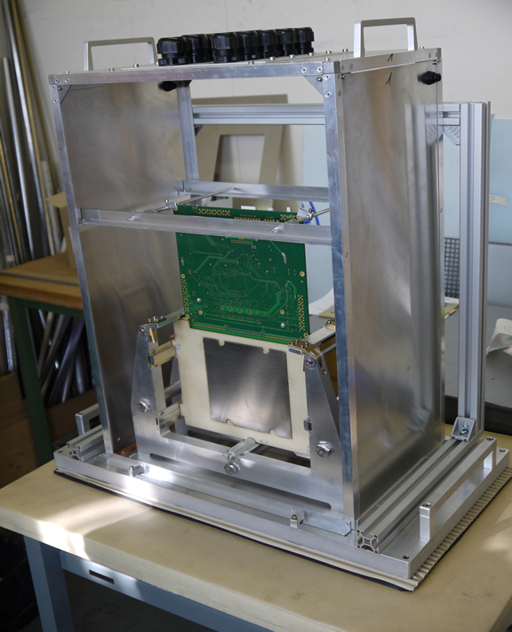
\includegraphics[width=0.6\columnwidth,]{Calorimeter/FCAL/figs/mechanical_structure_2}
    \caption{Photograph of the flexible mechanical structure. Tungsten absorber plates, glued on permaglass frames, are put into slots of the
rod assembly.}
    \label{fig:mechanical_structure}
\end{figure}
The flatness of the absorber plates is better than \SI{50}{\micro\meter} to allow for highly compact 
packing of sensor and absorber plates. This stack will be completed 
with absorber plates of the necessary quality up to a total thickness of 30 radiation lengths.

\subsection{Test-beam Measurements}

Test-beams were used to continue radiation hardness studies and study partly instrumented calorimeter prototypes. 
Calorimeter prototypes are built of tungsten absorber plates interspersed with detector  planes as described below. Detector planes comprise a sensor, Kapton fan-outs and FE ASICs.
The first milestones were the measurements in the test-beam of a four
detector plane prototype~\cite{Abramowicz:2017cer} and of a six detector plane prototype~\cite{Abramowicz:2018vwb}. 
Recently, measurements have been performed with a stack instrumented with 11 detector planes, out of which 3 have been operated with the FLAME readout.   

\subsubsection{Radiation Damage Studies}

Two studies of the radiation tolerance of potential BeamCal sensors have
been carried out.
In the first study, the radiation tolerance of prototype GaAs sensors
has been explored by
exposing the sensors to direct radiation from a high-intensity electron
beam of
about \SI{10}{MeV}, which is typical of the energy expected from
beamstrahlung
remnants at ILC. It was found that the sensors can be operated at
room temperature up
to approximately \SI{1}{MGy} without a significant increase in the
leakage current~\cite{1748-0221-7-11-P11022}; however, significant loss
in the response
to ionizing particles was observed. This loss can be partially
compensated, however,
by increasing the bias voltage. In addition, a new round of GaAs:Fe
prototype production
includes a small dopant concentration of iron, which is expected to mitigate
radiation damage effects. Characterization of these new prototypes is
expected soon.

In the second study~\cite{Anderson:2017kkq}, several different
solid-state sensor
technologies were
exposed to varying levels of radiation induced by electrons from the
SLAC End Station A
Test Beam (ESTB).
For this study, the ESTB test beam, with energies varying between 3
and \SI{15}{GeV}, was
directed into a tungsten beam stop. The beam stop was split at the depth
of the shower maximum
and the sensor inserted,
leading to an exposure incorporating the full spectrum of particle
species that will
irradiate the BeamCal sensors. Silicon diode and bulk GaAs, Sapphire and
SiC sensors
were exposed to doses of up to \SI{6}{MGy} of ionizing radiation, along with the
attendant dose of non-ionizing hadronic radiation associated with the
electromagnetic
shower. For GaAs, observed charge collection loss was similar to that of
the first study, although a room-temperature leakage current of
order \SI{10}{\micro\ampere\per\centi\meter\squared}
was observed for \SI{1}{MGy}-scale doses for a sensor
bias of \SI{600}{V}. No significant leakage current was observed for SiC
and Sapphire sensors
irradiated to \SI{0.8}{MGy} and \SI{3}{MGy}, respectively. For these doses, the
charge-collection
loss in SiC was approximately 50\% and for Sapphire, which has low
charge collection
even before irradiation, approximately 75\%. Observed charge
collection loss was
somewhat better for silicon diode sensors: a p-type, float-zone sensor
irradiated
to \SI{6}{MGy} experienced less than 40\% charge-collection loss. However, the silicon
diode sensors developed a significant leakage current. After
beneficial annealing, leakage currents of several hundred \si{\micro\ampere\per\centi\meter\squared}
per MGy of exposure were observed for room-temperature operation at full
depletion
voltage. Lowering the operating temperature to -30\textdegree C reduced
the leakage
current by over two orders of magnitude.
A study~\cite{Schumm:2018phi}
based on a simulation of the BeamCal radiation field
making use of the FLUKA Monte Carlo\cite{Bohlen:2014buj,Ferrari:2005zk}, and damage coefficients
determined from the ESTB results, estimated the accumulated power draw
for a BeamCal instrumented with silicon diode sensors operated
at -30\textdegree C
would be less than \SI{10}{W} per year of operation.

\subsubsection{Performance of a Prototype Calorimeter}

Prototypes of detector planes assembled with FE and ADC ASIC,
as shown in Figure~\ref{fig:fcal_lumical_module_photo},
were built using LumiCal and BeamCal sensors~\cite{1748-0221-7-01-T01004}, and successfully operated in 
test-beam~\cite{Abramowicz:2014gdq}.
\begin{figure}
    \centering
    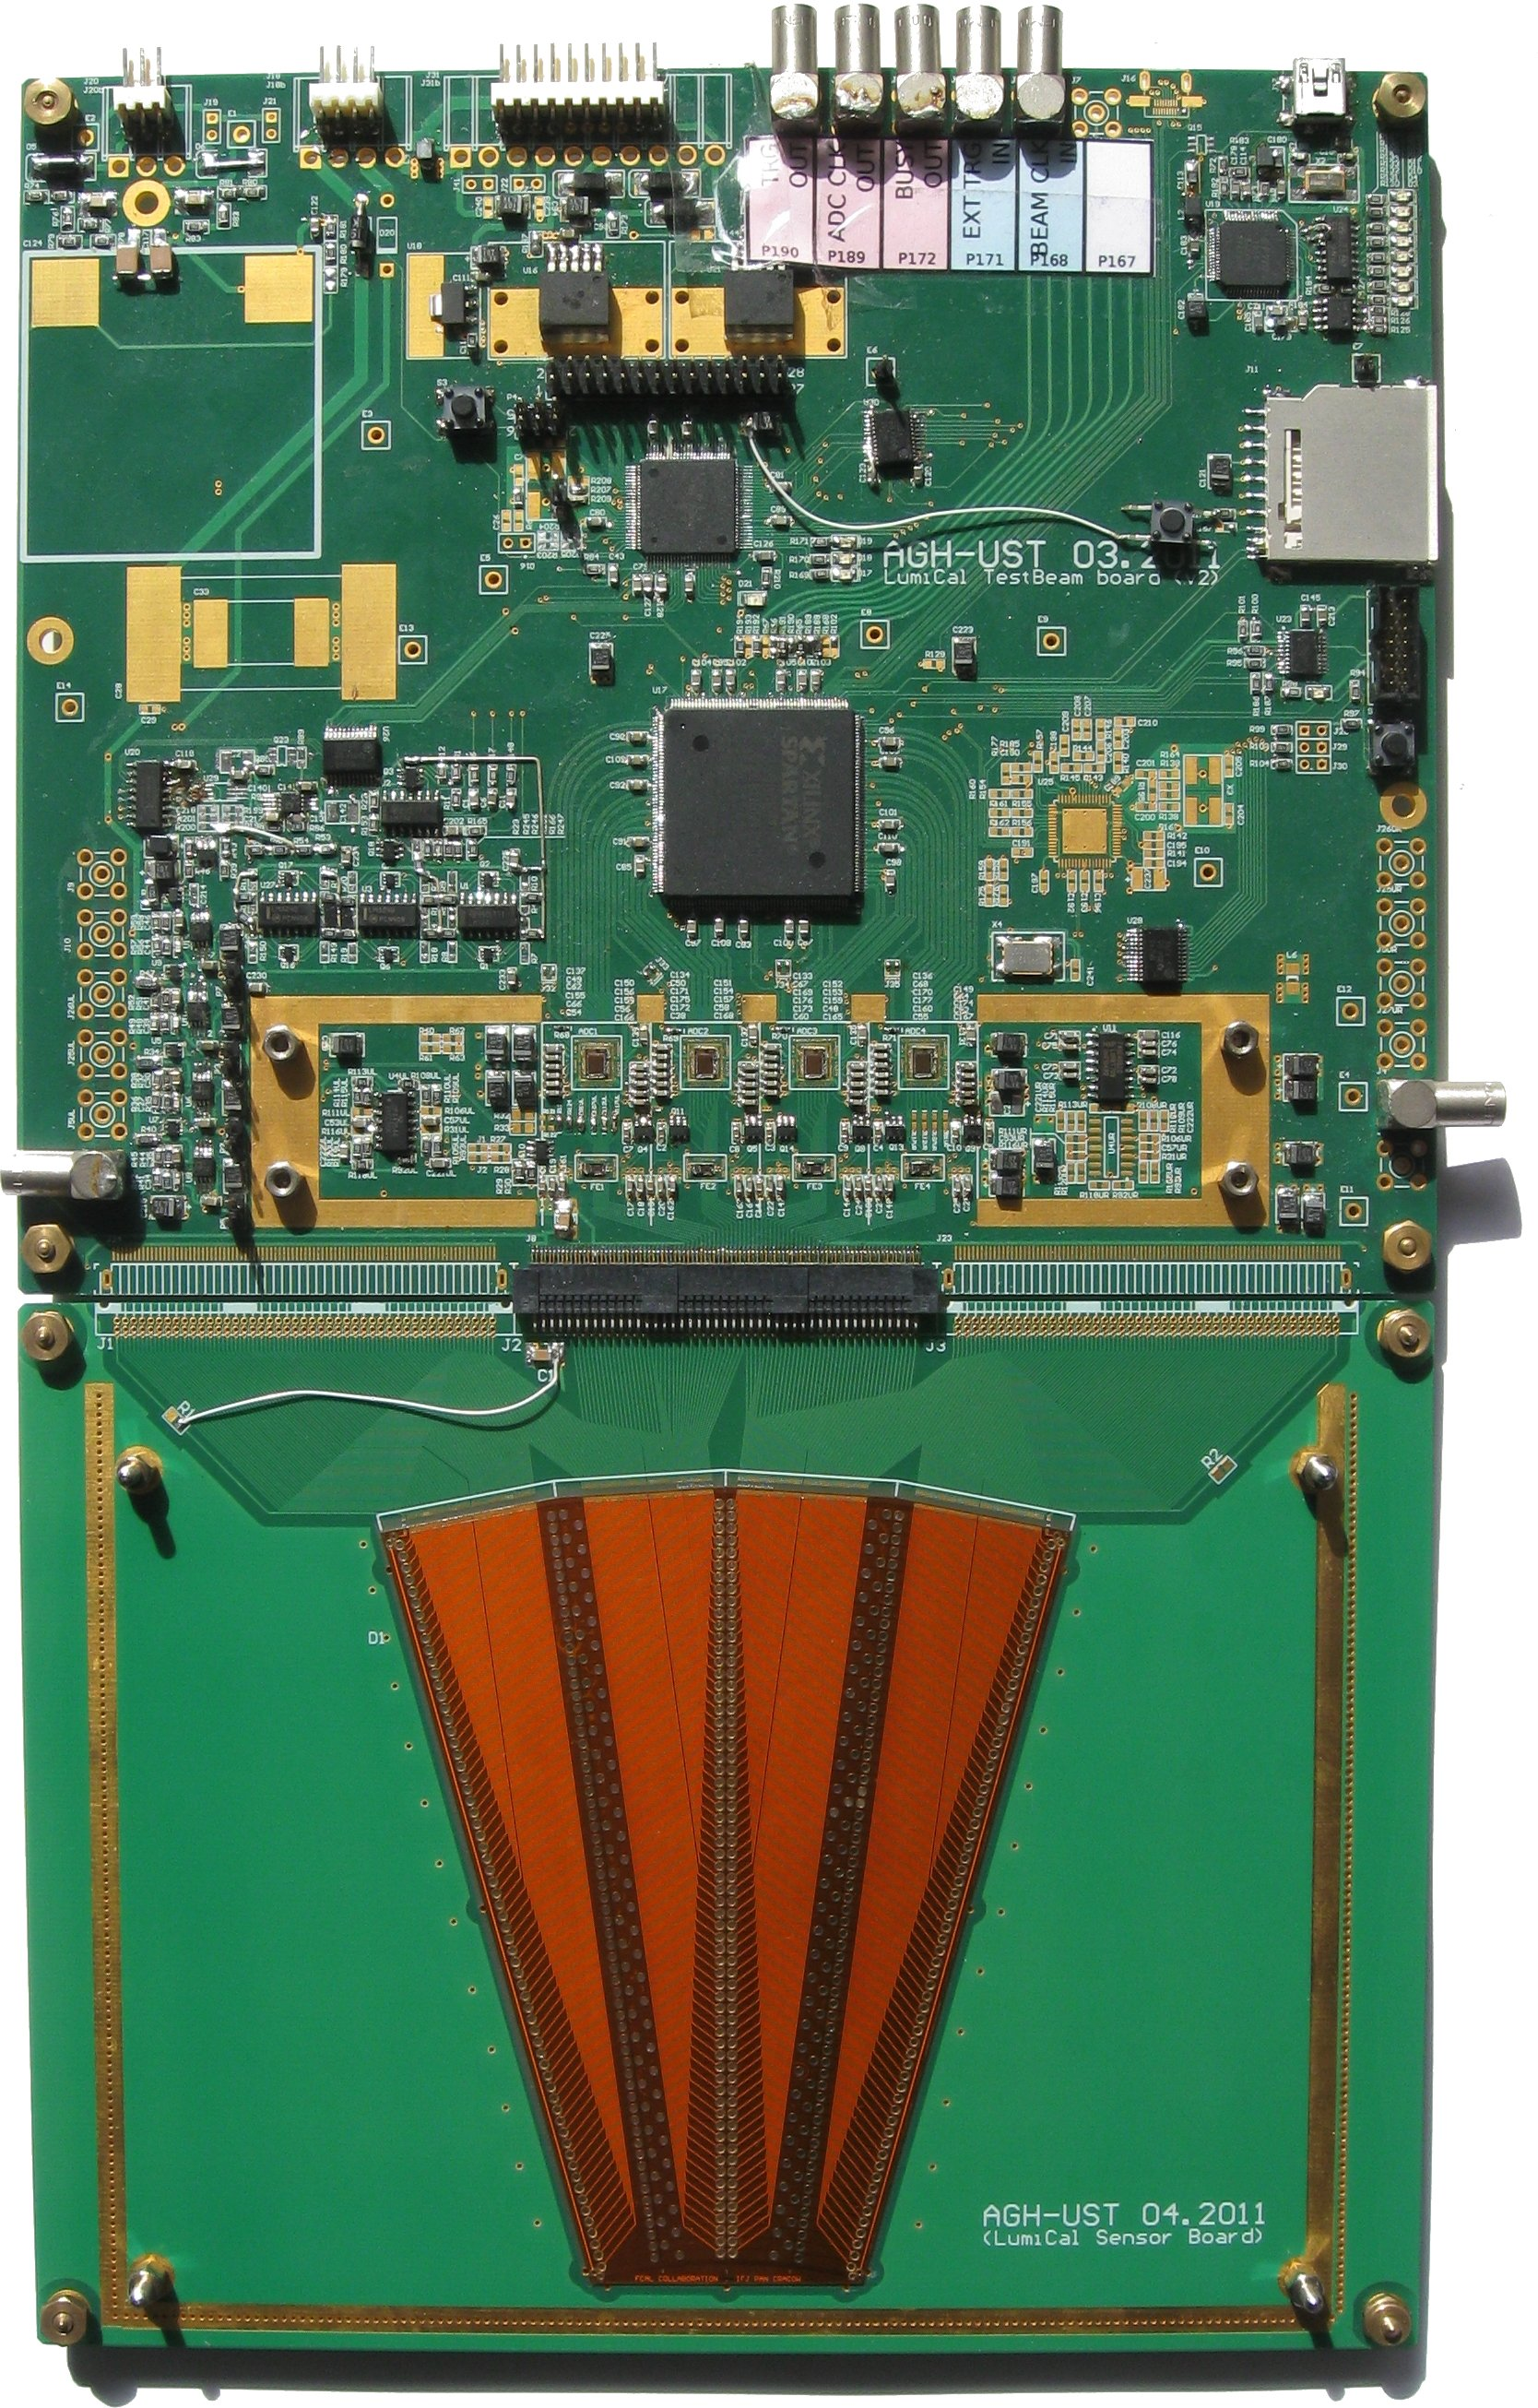
\includegraphics[width=0.35\columnwidth,angle=90]{Calorimeter/FCAL/figs/tb3_complete_module}
    \caption{Photograph of a fully instrumented detector plane for FCAL.}
    \label{fig:fcal_lumical_module_photo}
\end{figure}
In the next step four detector planes using silicon sensors were used to
study the performance of a prototype calorimeter in an electron and a muon beam. Different numbers of uniform
absorber plates were positioned in front and in between the detector planes in each
run, allowing to study the longitudinal and lateral shower development.
This first prototype, due to the large thickness of the instrumented readout boards, was not as compact as finally needed, but
allowed the demonstration that the multilayer operation and readout is successful. In addition, very good
agreement between data and Monte Carlo simulation
was obtained in the lateral and longitudinal shower development and the precision of the shower position reconstruction. The Moli\`ere 
radius was measured to be \SI{24.0(17)}{mm}.
\begin{figure}
    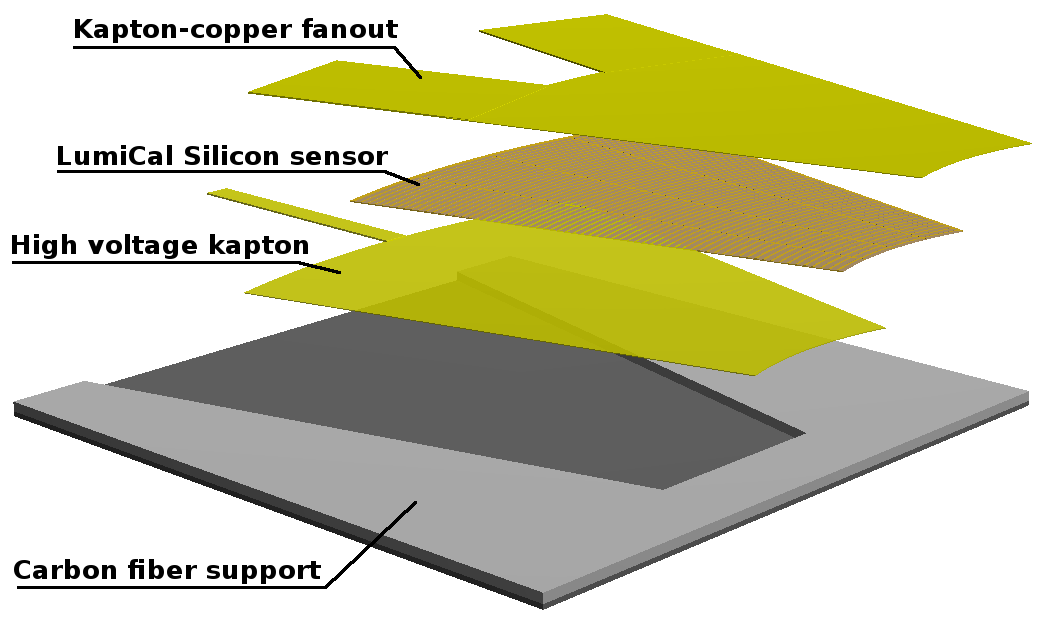
\includegraphics[width=0.99\columnwidth]{Calorimeter/FCAL/figs/lc_assembly_1.png}
    \caption{Thin LumiCal module assembly. The thickness of adhesive layers (not shown) between components is within \SIrange{10}{15}{\micro\meter}. The total thickness is \SI{650}{\micro\meter}.}
    \label{fig_ThinLCAssembly}
\end{figure}

In following test-beam campaigns eight thin detector planes, as shown in  Figure~\ref{fig_ThinLCAssembly}, 
interspersed by tungsten absorbers of 1 radiation length
thickness were used. The sensors were read out, as an intermediate solution, using 
the APV25 chip~\cite{949881,French2001359} hybrid board. It has 128 channels and two boards read a whole LumiCal sensor. 
Capacitive 
charge dividers were used to enlarge the dynamic range of the APV25 chip.  
The powering circuits and the fan-out part which connects silicon sensor pads with the front-end
board inputs were made from flexible Kapton-copper foils with thickness of \SI{70}{\micro\meter} for the high voltage one,
applied to the back n-side of the sensor and about \SI{120}{\micro\meter} for the fan-out.
Ultrasonic wire bonding was used to connect conductive traces on the fan-out to the sensor pads.
A support structure made of carbon fiber composite with a thickness of \SI{100}{\micro\meter} in the sensor-gluing area
provides mechanical stability. 
The ultrasonic wire bonding proved to provide good electrical performance, but for a detector plane thinner than \SI{1}{mm}, the wire loops,
which are typically \SIrange{100}{200}{\micro\meter} high, cause a serious problem when the module needs to be installed in a \SI{1}{mm} gap between absorber plates.
The bonding machine was tuned to make the loop as low as possible and technically acceptable.
The sampling based measurements, which were done using a con-focal laser scanning microscope, show that the loop
height is in the range \SIrange{50}{100}{\micro\meter}. The total thickness of the detector plane was \SI{650}{\micro\meter}.

The calorimeter prototype was studied in a \SIrange{1}{5}{GeV} electron beam at DESY~\cite{Ghenescu:2018sow,Abramowicz:2018vwb}. The shower position was reconstructed with a resolution of \SI{440(20)}{\micro\meter}.
The average transverse shower profile is shown in 
Figure~\ref{MR_5GeV} for data and Monte Carlo simulation. Very good agreement is found. The effective Moli\`ere radius is
determined to be \SI{8.1(3)}{mm} in data and \SI{8.4(1)}{mm} in Monte Carlo simulations.

\begin{figure}
    \centering
    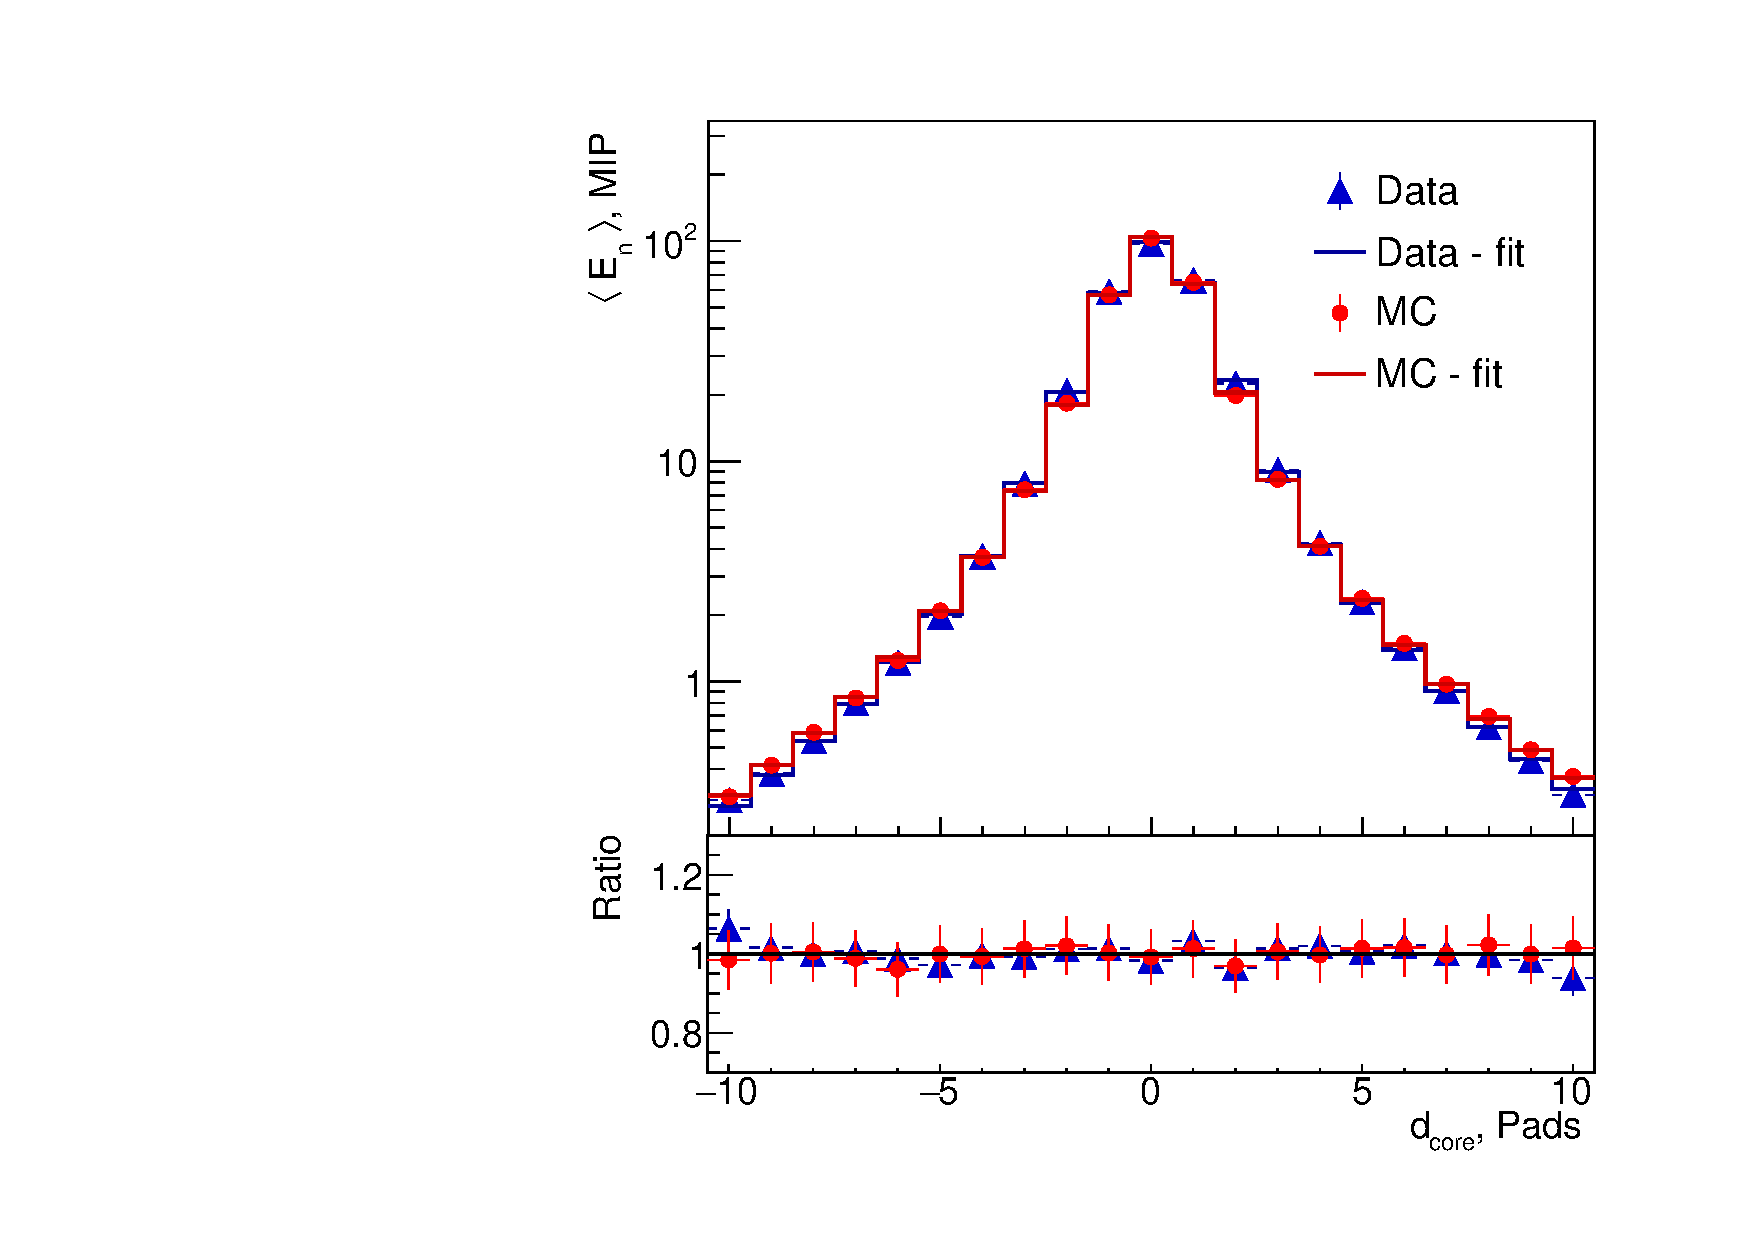
\includegraphics[width=\textwidth]{Calorimeter/FCAL/figs/MR_5GeV_EffS_v3.pdf}
    \caption{The average transverse shower profile, $\langle E^{det}_{n} \rangle$, as a function 
of the distance from the core, $d_{core}$, in units of pads, for data (blue triangles) and MC 
simulation (red circles). The histograms are the results of fits to data and MC using a parametrisation of the 
shower shape. The lower part of the figure shows the ratio 
of the distributions to the fitted function, for the data (blue) and the MC (red).}
    \label{MR_5GeV}
\end{figure}
In a recent test-beam campaign part of the calorimeter prototype was equipped with FLAME read-out boards and an FPGA data concentrator. Several millions events have been recorded in the same electron beam mentioned above. The data analysis is still ongoing.

\subsection{Engineering Challenges}
Engineering challenges within the current and future research of FCAL are the following:
\begin{itemize}
\item A slim assembled detector plane. First prototypes of a ultra-thin detector planes have been successfully
manufactured and used in test-beam measurements.
These technologies need to be completed and transferred into mass production. 
\item Miniaturized PCBs using FLAME chips, to be applicable in an experiment 
\item Development of readout ASICs for BeamCal.
Here prototypes are designed, and a submission is planned soon.
\item Operation using power pulsing to avoid active cooling.
\item A dedicated solution for data concentration, data reduction and transmission, allowing read out of 
the full calorimeters after each bunch crossing.
\item Precise alignment and position monitoring. The inner radius of LumiCal has to be controlled with a precision
of about \SI{10}{\micro\meter}, and the distance between the 
calorimeters on both sides of the IP with a precision of \SI{100}{\micro\meter}.
\item Montage and demontage of the calorimeters must be done when the beam-pipe is installed. The calorimeters must be segmented at 
least in two half cylinders, and corresponding auxiliary mechanics has to be developed.
\end{itemize}

\subsection{Future Plans}

\subsubsection{Novel Sensor Materials}

The performance of single crystal Sapphire sensors to detect minimum ionising particles has been studied for the 
first time~\cite{1748-0221-10-08-P08008}. Sapphire sensors are a promising alternative for GaAs to instrument
the region near the beam-pipe where a high radiation field is expected.

With Hamamatsu Photonics the design of 
edge-less silicon sensors is under preparation. Using edge-less sensors in LumiCal would avoid performance losses 
in gaps between sensor segments.

\subsubsection{Technological Calorimeter Prototype}

Currently the goal of FCAL is to prepare a full depth calorimeter prototype instrumented with more than 20
detector planes equipped with FLAME read-out for test-beam measurements. These measurements
are essential firstly to develop and test engineering solutions to build a very compact calorimeter and
secondly to verify the results of Monte Carlo studies. Depending on the test beam
results the calorimeter may be redesigned.
For the prototype calorimeter
a mechanical structure, a sufficient amount of ASICs, FPGAs for
data concentration and
a data acquisition system are needed. In addition, 
two-planes of a pixel tracker in front of LumiCal will be prepared to improve the polar angle resolution.

\subsubsection{Alignment and Position Monitoring }

A laboratory set-up for position monitoring has been constructed by IFJPAN Cracow using semi-transparent
silicon sensors~\cite{EUDETREPORT-2008-05}. Test measurements demonstrated that position monitoring 
with \si{\micro\meter} precision is possible. A design how to integrate the system in a larger detector has still to be developed. 

\subsubsection{Front-End and ADC ASICs}

Engineering solutions for a miniaturized FLAME readout boards will be developed, and an amount of ASICs will be fabricated
to be used in the larger calorimeter prototype.

A dedicated ASIC development is ongoing for BeamCal~\cite{6200898}
with a special option for a fast readout of a reduced amount of
information from a few bunch-crossings to be used for a fast feedback system for beam-tuning~\cite{1748-0221-3-10-P10004}.
A small prototype of a pixel sensor readout for the pair monitor, positioned in front of BeamCal was designed in SoI
technology~\cite{Sato201153}. This development is foreseen to be continued.

\subsubsection{Data Acquisition}

Ongoing further work will focus on the ethernet transmission.The higher level DAQ will depend on the functionality of the 
data concentrator. For the readout of test-beam data software is developed, mainly by the University of Tel Aviv,
which can be easily adopted. For the final device FCAL will follow the developments of a common DAQ for all detectors.
